\documentclass[xetex,mathserif,serif]{beamer}
\usepackage{polyglossia}
\setdefaultlanguage[babelshorthands=true]{russian}
\usepackage{minted}
\usepackage{tabu}

\useoutertheme{infolines}

\usepackage{fontspec}
\setmainfont{FreeSans}
\newfontfamily{\russianfonttt}{FreeSans}

\definecolor{links}{HTML}{2A1B81}
\hypersetup{colorlinks,linkcolor=,urlcolor=links}

\tabulinesep=0.7mm

\title{Распределённые приложения, gRPC}
\author[Юрий Литвинов]{Юрий Литвинов \newline \textcolor{gray}{\small\texttt{yurii.litvinov@gmail.com}}}

\date{13.05.2020г}

\begin{document}
    
    \frame{\titlepage}

    \section{protobuf}

    \begin{frame}
        \frametitle{Protocol buffers}
        \framesubtitle{protobuf}
        \begin{itemize}
            \item Механизм сериализации-десериализации данных
            \item Компактное бинарное представление
            \item Декларативное описание формата данных, генерация кода для языка программирования
            \begin{itemize}
                \item Поддерживается Java, C\#, Python, C++, Objective-C, Go, Ruby, ...
            \end{itemize}
            \item Бывает v2 и v3, с некоторыми синтаксическими отличиями
            \item Хитрый протокол передачи, \url{https://developers.google.com/protocol-buffers/docs/encoding}
            \begin{itemize}
                \item Base 128 varint-ы
                \item До 10 раз компактнее XML 
            \end{itemize}
        \end{itemize}
    \end{frame}

    \begin{frame}[fragile]
        \frametitle{Пример}
        Файл .proto:
        \begin{minted}{protobuf}
message Person {
  required string name = 1;
  required int32 id = 2;
  optional string email = 3;
}
        \end{minted}
        Файл .java:
        \begin{minted}{java}
Person john = Person.newBuilder()
    .setId(1234)
    .setName("John Doe")
    .setEmail("jdoe@example.com")
    .build();
output = new FileOutputStream(args[0]);
john.writeTo(output);
        \end{minted}
    \end{frame}

    \begin{frame}
        \frametitle{Технические подробности}
        Для Java:
        \begin{itemize}
            \item .proto-файлы --- в папку src/main/proto
            \item gradle-плагин com.google.protobuf
            \item \url{https://github.com/google/protobuf-gradle-plugin/blob/master/examples/exampleProject/build.gradle}
        \end{itemize}
        Для остального: скачать и поставить protoc
        \begin{itemize}
            \item \url{https://github.com/google/protobuf}
        \end{itemize}
    \end{frame}

    \section{gRPC}

    \begin{frame}
        \frametitle{gRPC}
        \begin{columns}
            \begin{column}{0.6\textwidth}
                \begin{itemize}
                    \item Средство для удалённого вызова (RPC)
                    \item Работает поверх protobuf
                    \item Разрабатывается Google
                    \item Поддерживает Java, C\#, C++, Python,  Objective-C, Go, Ruby, ...
                \end{itemize}
            \end{column}
            \begin{column}{0.4\textwidth}
                \begin{center}
                    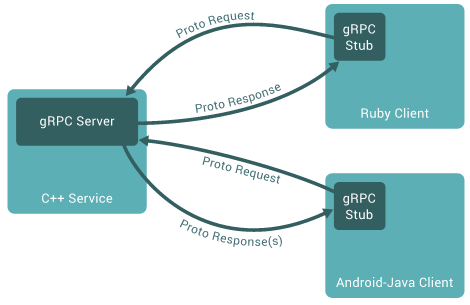
\includegraphics[width=\textwidth]{grpc.png}
                \end{center}
            \end{column}
        \end{columns}
    \end{frame}

    \begin{frame}[fragile]
        \frametitle{Технические подробности}
        \begin{itemize}
            \item Сервисы описываются в том же .proto-файле, что и протокол protobuf-а
            \item В качестве типов параметров и результатов --- message-и protobuf-а
        \end{itemize}
        \begin{minted}{protobuf}
service RouteGuide {
  rpc GetFeature(Point) returns (Feature) {}
  rpc ListFeatures(Rectangle) returns (stream Feature) {}
  rpc RecordRoute(stream Point) returns (RouteSummary) {}
  rpc RouteChat(stream RouteNote) returns (stream RouteNote) {}
}
        \end{minted}
        \begin{itemize}
            \item Сборка --- плагином grpc к protoc
        \end{itemize}
    \end{frame}

    \begin{frame}[fragile]
        \frametitle{Реализация сервиса на Java}
        \begin{scriptsize}
            \begin{minted}{java}
private static class RouteGuideService extends RouteGuideGrpc.RouteGuideImplBase {
    ...
    @Override
    public void getFeature(Point request, StreamObserver<Feature> responseObserver) {
      responseObserver.onNext(checkFeature(request));
      responseObserver.onCompleted();
    }

    @Override
    public void listFeatures(Rectangle request, StreamObserver<Feature> responseObserver) {
      for (Feature feature : features) {
        ...
        int lat = feature.getLocation().getLatitude();
        int lon = feature.getLocation().getLongitude();
        if (lon >= left && lon <= right && lat >= bottom && lat <= top) {
          responseObserver.onNext(feature);
        }
      }
      responseObserver.onCompleted();
    }
            \end{minted}
        \end{scriptsize}
    \end{frame}

    \begin{frame}[fragile]
        \frametitle{Реализация сервиса на Java (2)}
        \begin{scriptsize}
            \begin{minted}{java}
    @Override
    public StreamObserver<RouteNote> routeChat(
            final StreamObserver<RouteNote> responseObserver) {
      return new StreamObserver<RouteNote>() {
        @Override
        public void onNext(RouteNote note) {
          List<RouteNote> notes = getOrCreateNotes(note.getLocation());
          for (RouteNote prevNote : notes.toArray(new RouteNote[0])) {
            responseObserver.onNext(prevNote);
          }
          notes.add(note);
        }
        @Override
        public void onError(Throwable t) {
          logger.log(Level.WARNING, "routeChat cancelled");
        }
        @Override
        public void onCompleted() {
          responseObserver.onCompleted();
        }
      };
    }
            \end{minted}
        \end{scriptsize}
    \end{frame}

    \begin{frame}[fragile]
        \frametitle{Что написать в build.gradle}
        \begin{small}
            \begin{minted}{groovy}
protobuf {
    protoc {
        artifact = "com.google.protobuf:protoc:3.11.0"
    }
    plugins {
        grpc {
            artifact = 'io.grpc:protoc-gen-grpc-java:1.30.0-SNAPSHOT'
        }
    }
    generateProtoTasks {
        all()*.plugins {
            grpc {
                outputSubDir = 'java'
            }
        }
    }
    generatedFilesBaseDir = "$projectDir/src"
}
            \end{minted}
        \end{small}
    \end{frame}

    \begin{frame}[fragile]
        \frametitle{Запуск сервиса}
        \begin{footnotesize}
            \begin{minted}{java}
private void start() throws IOException {
    int port = 50051;
    server = ServerBuilder.forPort(port)
        .addService(new GreeterImpl())
        .build()
        .start();
    logger.info("Server started, listening on " + port);
    Runtime.getRuntime().addShutdownHook(new Thread() {
        @Override
        public void run() {
            System.err.println("*** shutting down gRPC server since JVM is shutting down");
            HelloWorldServer.this.stop();
            System.err.println("*** server shut down");
      }
    });
}
            \end{minted}
        \end{footnotesize}
    \end{frame}

    \begin{frame}[fragile]
        \frametitle{Инициализация клиента}
        \begin{minted}{java}
public HelloWorldClient(String host, int port) {
    this(ManagedChannelBuilder.forAddress(host, port)
        .usePlaintext()
        .build());
}
        \end{minted}
        \vspace{5mm}
        \url{https://github.com/grpc/grpc-java/blob/master/examples/src/main/java/io/grpc/examples/helloworld/HelloWorldClient.java}
    \end{frame}

    \section{Задача}

    \begin{frame}
        \frametitle{Задание на пару}
        \begin{footnotesize}
            В командах по два человека разработать сетевой чат (наподобие Telegram) с помощью gRPC
            \begin{itemize}
                \item peer-to-peer, то есть соединение напрямую
                \begin{itemize}
                    \item Одно и то же приложение может быть и клиентом, и сервером
                \end{itemize}
                \item Консольный пользовательский интерфейс
                \begin{itemize}
                    \item Отображение имени отправителя, даты и времени отправки и текста сообщения
                \end{itemize}
                \item При запуске указываются:
                \begin{itemize}
                    \item Адрес peer-а и порт, если хотим подключиться
                    \begin{itemize}
                        \item Должно быть можно не указывать, тогда работаем в режиме сервера
                    \end{itemize}
                    \item Своё имя пользователя
                \end{itemize}
                \item Пишем адрес репозитория сюда: \url{https://forms.gle/NKEQKuJ2HAa8syhM7}
                \item За 10 минут до конца собираемся в общий чат и показываем, что получилось
            \end{itemize}
        \end{footnotesize}
    \end{frame}

\end{document}